%%%%%%%%%%%%%%%%%%%%%%%%%%%%%%%%%%%%%%%%%
% Beamer Presentation
% LaTeX Template
% Version 1.0 (10/11/12)
%
% This template has been downloaded from:
% http://www.LaTeXTemplates.com
%
% License:
% CC BY-NC-SA 3.0 (http://creativecommons.org/licenses/by-nc-sa/3.0/)
%
%%%%%%%%%%%%%%%%%%%%%%%%%%%%%%%%%%%%%%%%%

%----------------------------------------------------------------------------------------
%	PACKAGES AND THEMES
%----------------------------------------------------------------------------------------

\documentclass{beamer}

\mode<presentation> {

% The Beamer class comes with a number of default slide themes
% which change the colors and layouts of slides. Below this is a list
% of all the themes, uncomment each in turn to see what they look like.

%\usetheme{default}
%\usetheme{AnnArbor}
%\usetheme{Antibes}
%\usetheme{Bergen}
%\usetheme{Berkeley}
%\usetheme{Berlin}
%\usetheme{Boadilla}
%\usetheme{CambridgeUS}
%\usetheme{Copenhagen}
%\usetheme{Darmstadt}
%\usetheme{Dresden}
%\usetheme{Frankfurt}
%\usetheme{Goettingen}
%\usetheme{Hannover}
%\usetheme{Ilmenau}
%\usetheme{JuanLesPins}
%\usetheme{Luebeck}
\usetheme{Madrid}
%\usetheme{Malmoe}
%\usetheme{Marburg}
%\usetheme{Montpellier}
%\usetheme{PaloAlto}
%\usetheme{Pittsburgh}
%\usetheme{Rochester}
%\usetheme{Singapore}
%\usetheme{Szeged}
%\usetheme{Warsaw}

% As well as themes, the Beamer class has a number of color themes
% for any slide theme. Uncomment each of these in turn to see how it
% changes the colors of your current slide theme.

%\usecolortheme{albatross}
\usecolortheme{beaver}
%\usecolortheme{beetle}
%\usecolortheme{crane}
%\usecolortheme{dolphin}
%\usecolortheme{dove}
%\usecolortheme{fly}
%\usecolortheme{lily}
%\usecolortheme{orchid}
%\usecolortheme{rose}
%\usecolortheme{seagull}
%\usecolortheme{seahorse}
%\usecolortheme{whale}
%\usecolortheme{wolverine}

%\setbeamertemplate{footline} % To remove the footer line in all slides uncomment this line
%\setbeamertemplate{footline}[page number] % To replace the footer line in all slides with a simple slide count uncomment this line

%\setbeamertemplate{navigation symbols}{} % To remove the navigation symbols from the bottom of all slides uncomment this line
}
% xtong's tools
% aliasis
\newcommand{\xemp}[1]{{\color{red}{\textbf{#1}}}}
\newcommand{\bs}{\boldsymbol}
\newcommand{\mean}[2]{\left\langle{#1}\right\rangle_{#2}}
\newcommand{\trb}[1]{\textrm{Tr}\left({#1}\right)}
\newcommand{\trs}[1]{\textrm{Tr}\left[{#1}\right]}
\newcommand{\invb}[1]{{\left({#1}\right)^-}}
\newcommand{\invs}[1]{{\left[{#1}\right]^-}}
\newcommand\numberthis{\addtocounter{equation}{1}\tag{\theequation}}
\renewcommand{\eqref}[1]{Eq.\,\ref{#1}}
%
% vectors and matrices
\newcommand{\va}{\mathbf{a}}
\newcommand{\vb}{\mathbf{b}}
\newcommand{\vc}{\mathbf{c}}
\newcommand{\vf}{\mathbf{f}}
\newcommand{\vg}{\mathbf{g}}
\newcommand{\vh}{\mathbf{h}}
\newcommand{\vv}{\mathbf{v}}
\newcommand{\vx}{\mathbf{x}}
\newcommand{\vu}{\mathbf{u}}
\newcommand{\vy}{\mathbf{y}}
\newcommand{\vw}{\mathbf{w}}
\newcommand{\vs}{\mathbf{s}}
% 
\newcommand{\xf}{\mathbf{F}}
\newcommand{\xg}{\mathbf{G}}
\newcommand{\xh}{\mathbf{H}}
\newcommand{\xk}{\mathbf{K}}
\newcommand{\xl}{\mathbf{L}}
\newcommand{\xr}{\mathbf{R}}
%
\newcommand{\xu}{\mathbf{U}}
\newcommand{\xv}{\mathbf{V}}
\newcommand{\xx}{\mathbf{X}}
\newcommand{\xw}{\mathbf{W}}
\newcommand{\xy}{\mathbf{Y}}
\newcommand{\xz}{\mathbf{Z}}
\newcommand{\xa}{\mathbf{A}}
\newcommand{\xd}{\mathbf{D}}
% 
% with tildes
%% vectors
\newcommand{\vat}{\tilde{\vb}}
\newcommand{\vbt}{\tilde{\vb}}
\newcommand{\vct}{\tilde{\vc}}
\newcommand{\vht}{\tilde{\vh}}
\newcommand{\vvt}{\tilde{\vv}}
\newcommand{\vst}{\tilde{\vs}}
\newcommand{\vut}{\tilde{\vu}}
\newcommand{\vft}{\tilde{\vf}}
\newcommand{\xut}{\tilde{\xu}}
\newcommand{\vxt}{\tilde{\vx}}
\newcommand{\xvt}{\tilde{\xv}}
\newcommand{\xyt}{\tilde{\xy}}
%% matrices
\newcommand{\xwt}{\tilde{\xw}}
%
% with hats
\newcommand{\vhh}{\hat{\vh}}
\newcommand{\xvh}{\hat{\xv}}
\newcommand{\vvh}{\hat{\vv}}
\newcommand{\vyh}{\hat{\vy}}
\newcommand{\vxh}{\hat{\vx}}
\newcommand{\vuh}{\hat{\vu}}
\newcommand{\vfh}{\hat{\vf}}
\newcommand{\xyh}{\hat{\xy}}
\newcommand{\xxh}{\hat{\xx}}
\newcommand{\xuh}{\hat{\xu}}
%
%
% derivatives
\newcommand{\DRV}[2]{\frac{d #1}{d #2}}
\newcommand{\DRC}[3]{\DRV{#1}{#2}\DRV{#2}{#3}}
\newcommand{\PDV}[2]{\frac{\partial #1}{\partial #2}}
\newcommand{\PDC}[3]{\PDV{#1}{#2}\PDV{#2}{#3}}
%
% the diagnal matrix
\newcommand{\id}{\textrm{\textbf{I}}}
\newcommand{\im}{\textrm{\textbf{I}}}
% the vector of ones
\newcommand{\one}{\mathbf{1}}
% 
% xiaoran's edit
\newcommand{\xadd}[1]{\textcolor{blue}{#1}}
\newcommand{\xdel}[1]{\textcolor{red}{\sout{#1}}}
\newcommand{\xrpl}[2]{\xdel{#1}\xadd{#2}}
\newcommand{\xacc}[1]{\textcolor{ForestGreen}{#1}}
%
%
% declarations
% argument of the minimum / maximum
\DeclareMathOperator*{\argmin}{arg\,min}
\DeclareMathOperator*{\argmax}{arg\,max}
%
% norms
\newcommand\norm[1]{\left\lVert#1\right\rVert}
\newcommand{\xmx}{\bs{X}}
\newcommand{\xmt}{\bs{X}^{\prime}}
\newcommand{\imx}{\bs{I}}
\newcommand{\umx}{\bs{U}}
\newcommand{\umt}{\bs{U}^{\prime}}
\newcommand{\yvc}{\bs{y}}
\newcommand{\yht}{\hat{\bs{y}}}
\usepackage{graphicx} % Allows including images
\usepackage{booktabs} % Allows the use of \toprule, \midrule and \bottomrule in tables

%----------------------------------------------------------------------------------------
%	TITLE PAGE
%----------------------------------------------------------------------------------------

\title[Kernel Genomics]{ML and REML v.s. MINQUE}

\author{Xiaoran Tong\\ Xiaoxi Shen \\ Qin Lu} % Your name
\institute[EPI Biosta, MSU] % Your institution as it will appear on the bottom of every slide, may be shorthand to save space
{
  Michigan State University \\ % Your institution for the title page
  \medskip
  \textit{tongxia1@msu.edu} \\% Your email address
  \textit{qlu@epi.msu.edu} % Your email address
}
\date{\today} % Date, can be changed to a custom date

\begin{document}

\begin{frame}
\titlepage % Print the title page as the first slide
\end{frame}

\begin{frame}
\frametitle{Table of Content} % Table of contents slide, comment this block out to remove it
\tableofcontents % Throughout your presentation, if you choose to use \section{} and \subsection{} commands, these will automatically be printed on this slide as an overview of your presentation
\end{frame}

%----------------------------------------------------------------------------------------
%	PRESENTATION SLIDES
%----------------------------------------------------------------------------------------
\section{Simulations}
\begin{frame}
\frametitle{Simulation Settings:}
\textbf{Data Generation:}
\begin{itemize}
\item Drawn from 1000 Genome Project (total sample size is 2504);
  \begin{itemize}
  \item N=1250, for both learning and evaluation;
  \item P=4000, SNPs of $MAF > 0.01$
  \end{itemize}
\item \% of functional variants = 10\%;
\item True Model: $y \sim \mathcal{N}(0, \epsilon \id + \sigma^2 \xv)$;
  \begin{itemize}
    \item size of noise, $\epsilon \in \{0.1, 0.2, 0.5, 1.0\}$
    \item true covariance, $\xv$:
      \begin{itemize}
      \item Gaussian Kernel: $d_{i,j}=\frac{1}{P} \exp{\frac{\norm{\vx_i, \vx_j}_2^2}{0.1}}$
      \item Product Kernel: $d_{i,j}=\vx_i^T \vx_j$
      \end{itemize}
  \end{itemize}
\item Distortion = \{sigmoid(y), sin(1 $\pi$ y), sin(2 $\pi$ y)\}
\end{itemize}
\end{frame}
%---------------------------------------------------------
\begin{frame}
  \frametitle{Simulation Settings:}
  \textbf{Learning and evaluation:}
  \begin{itemize}
  \item always use product kernel built from all $P$ genomic variants
    $\xg$ as the working covariance matrix
    \begin{itemize}
    \item $\xvh = \hat{\epsilon}\id + \hat{\sigma}^2 \xg^\prime \xg$
    \item $\hat{\sigma}^2$ and $\hat{\epsilon}$ are variance
      components to beestimated.
    \end{itemize}
  \item methods to be benchmarked: 
    \begin{itemize}
    \item GCTA-REML, R-ML;
    \item linear and polynomial MINQUE implemented by Rcpp and R;
    \end{itemize}
  \item mean square error for evaluating prediction performance,
    assuming $\vy$ to be normal (even for MINQUE):
    \begin{itemize}
    \item $\hat{y} = \xvh_G \xvh^- \vy$, where
      $\xvh_g = \hat{\sigma}^2\xg^\prime\xg$
    \item $MSE = \frac{1}{N} \norm{\vy, \hat{\vy}}_2^2$
    \end{itemize}
  \item to  compare efficiency, the runing time between creation
    of covariance matrix and prediction is used.
  \end{itemize}
\end{frame}
%---------------------------------------------------------
\begin{frame}{EXP 01: covariance mis-specification, MSE}
  \scriptsize{True covariance is a Gaussian kernel, working covariance is a product kernel}
  \normalsize
  \begin{figure}
    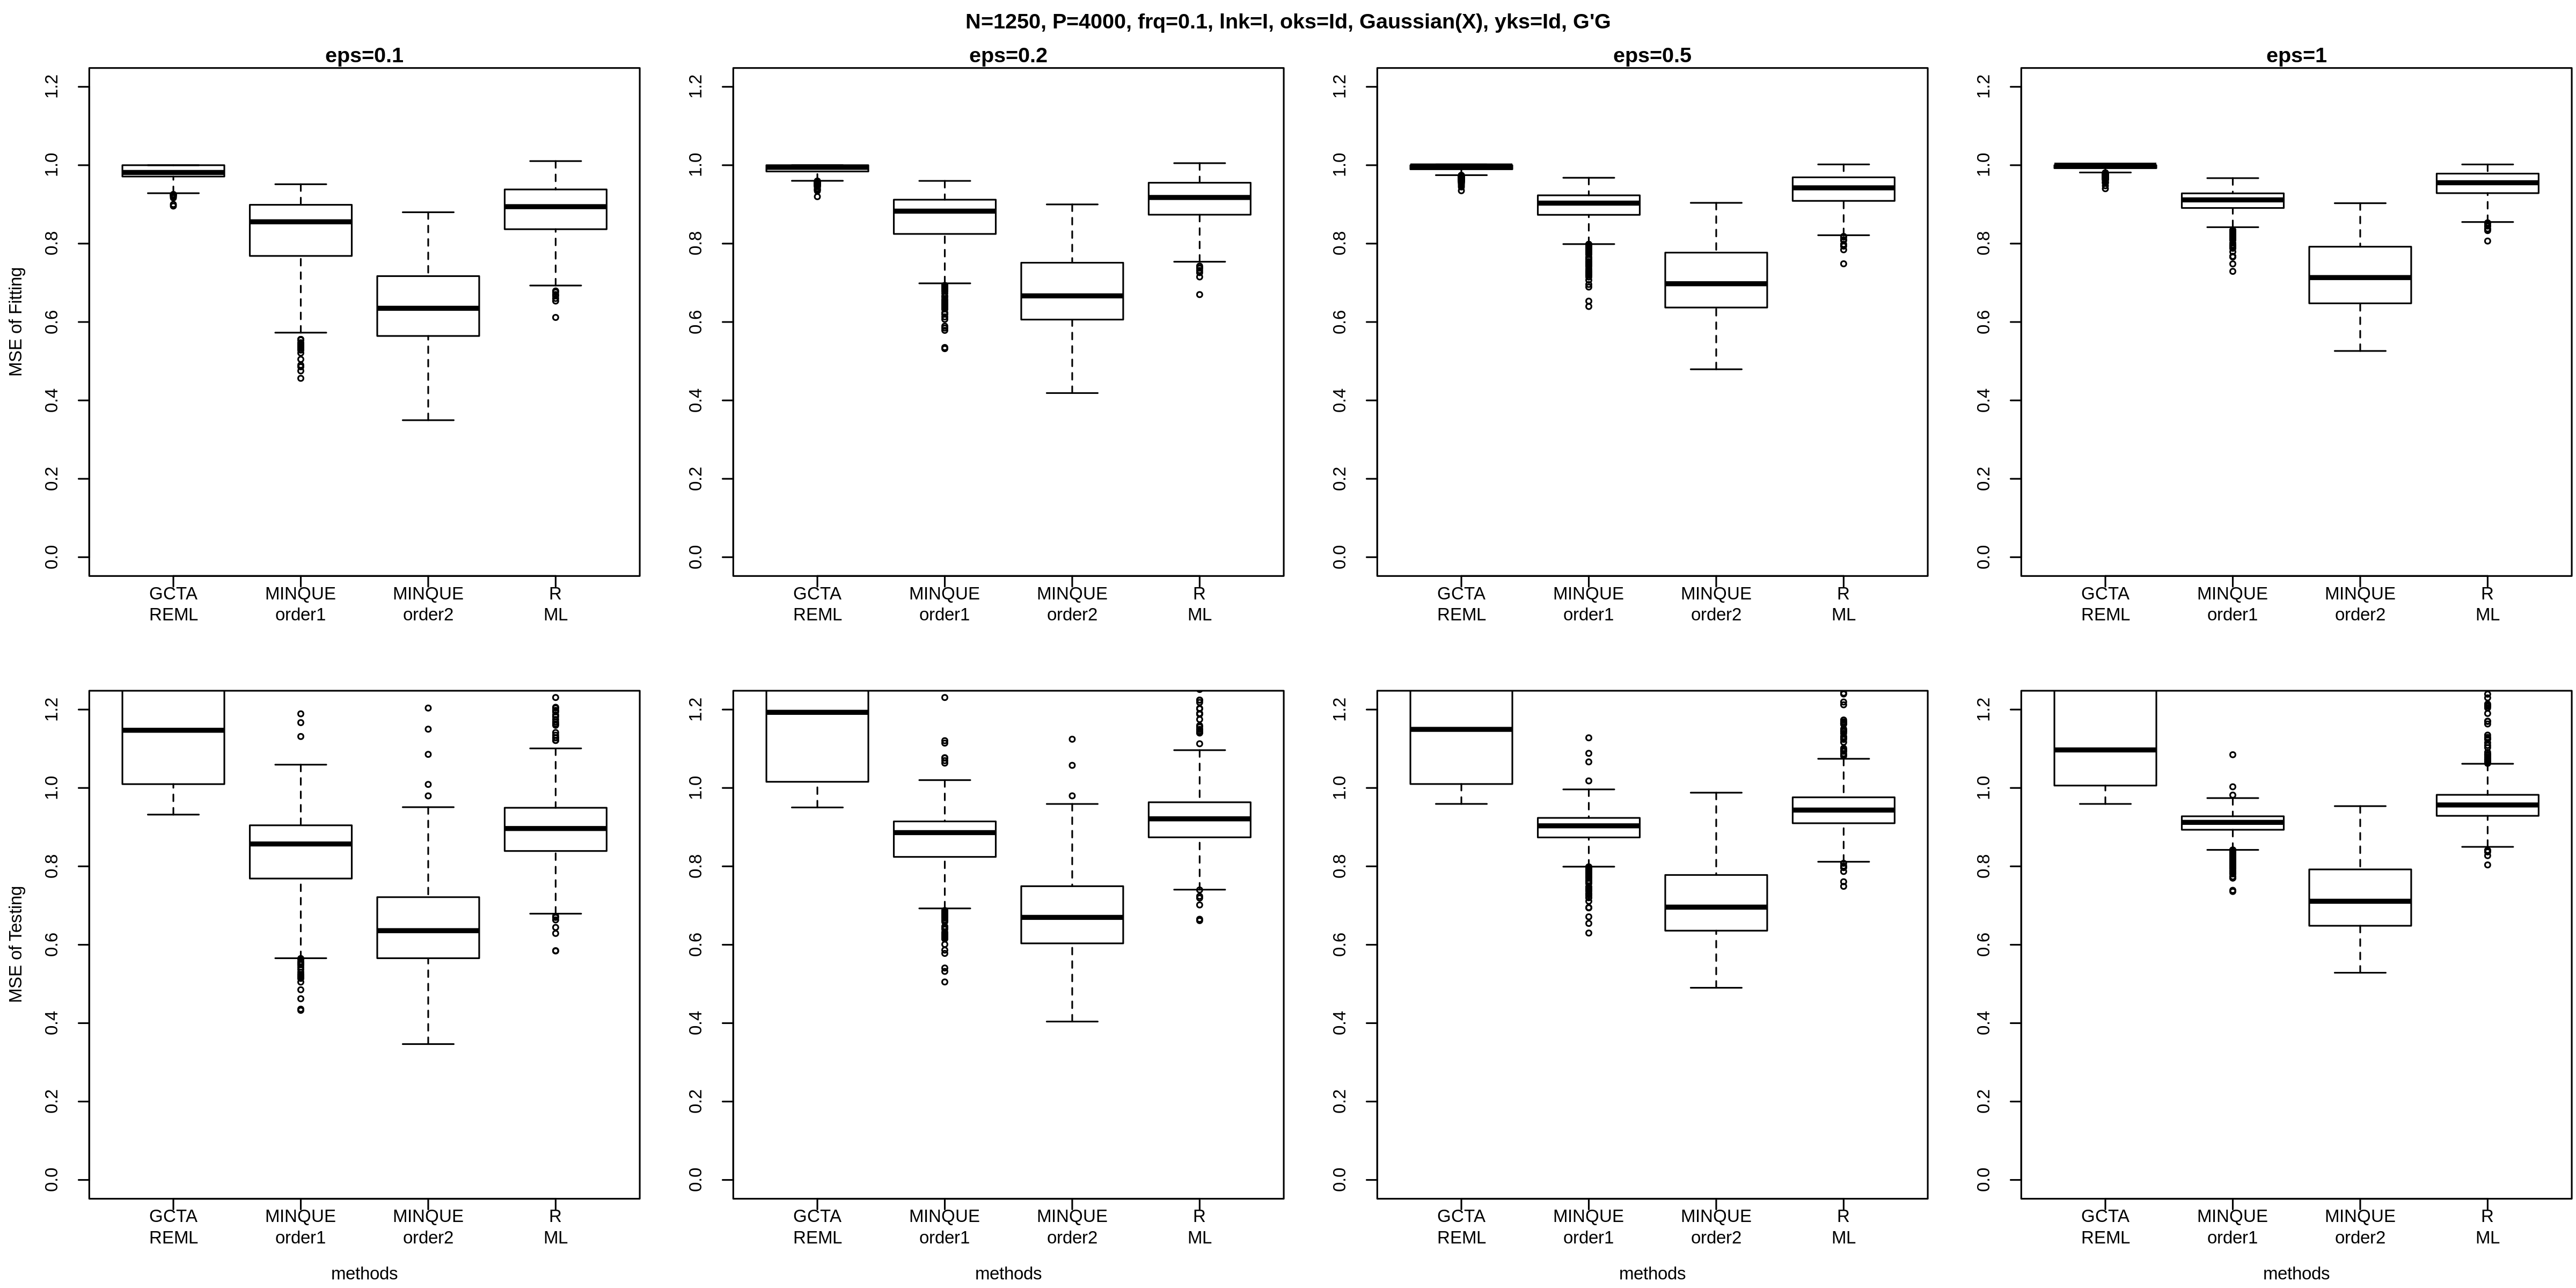
\includegraphics[width=1.00\linewidth]{s01_bxp.png}
  \end{figure}
\end{frame}
\begin{frame}{EXP 01: covariance mis-specification, RTM}
  \scriptsize{True covariance is a Gaussian kernel, working covariance is a product kernel}
  \normalsize
  \begin{figure}
    
\includegraphics[width=1.00\linewidth]{t01_bxp.png}
  \end{figure}
\end{frame}
% ---------------------------------------------------------
\begin{frame}{EXP 02: sigmoid distortion of $\vy$, MSE}
  \begin{figure}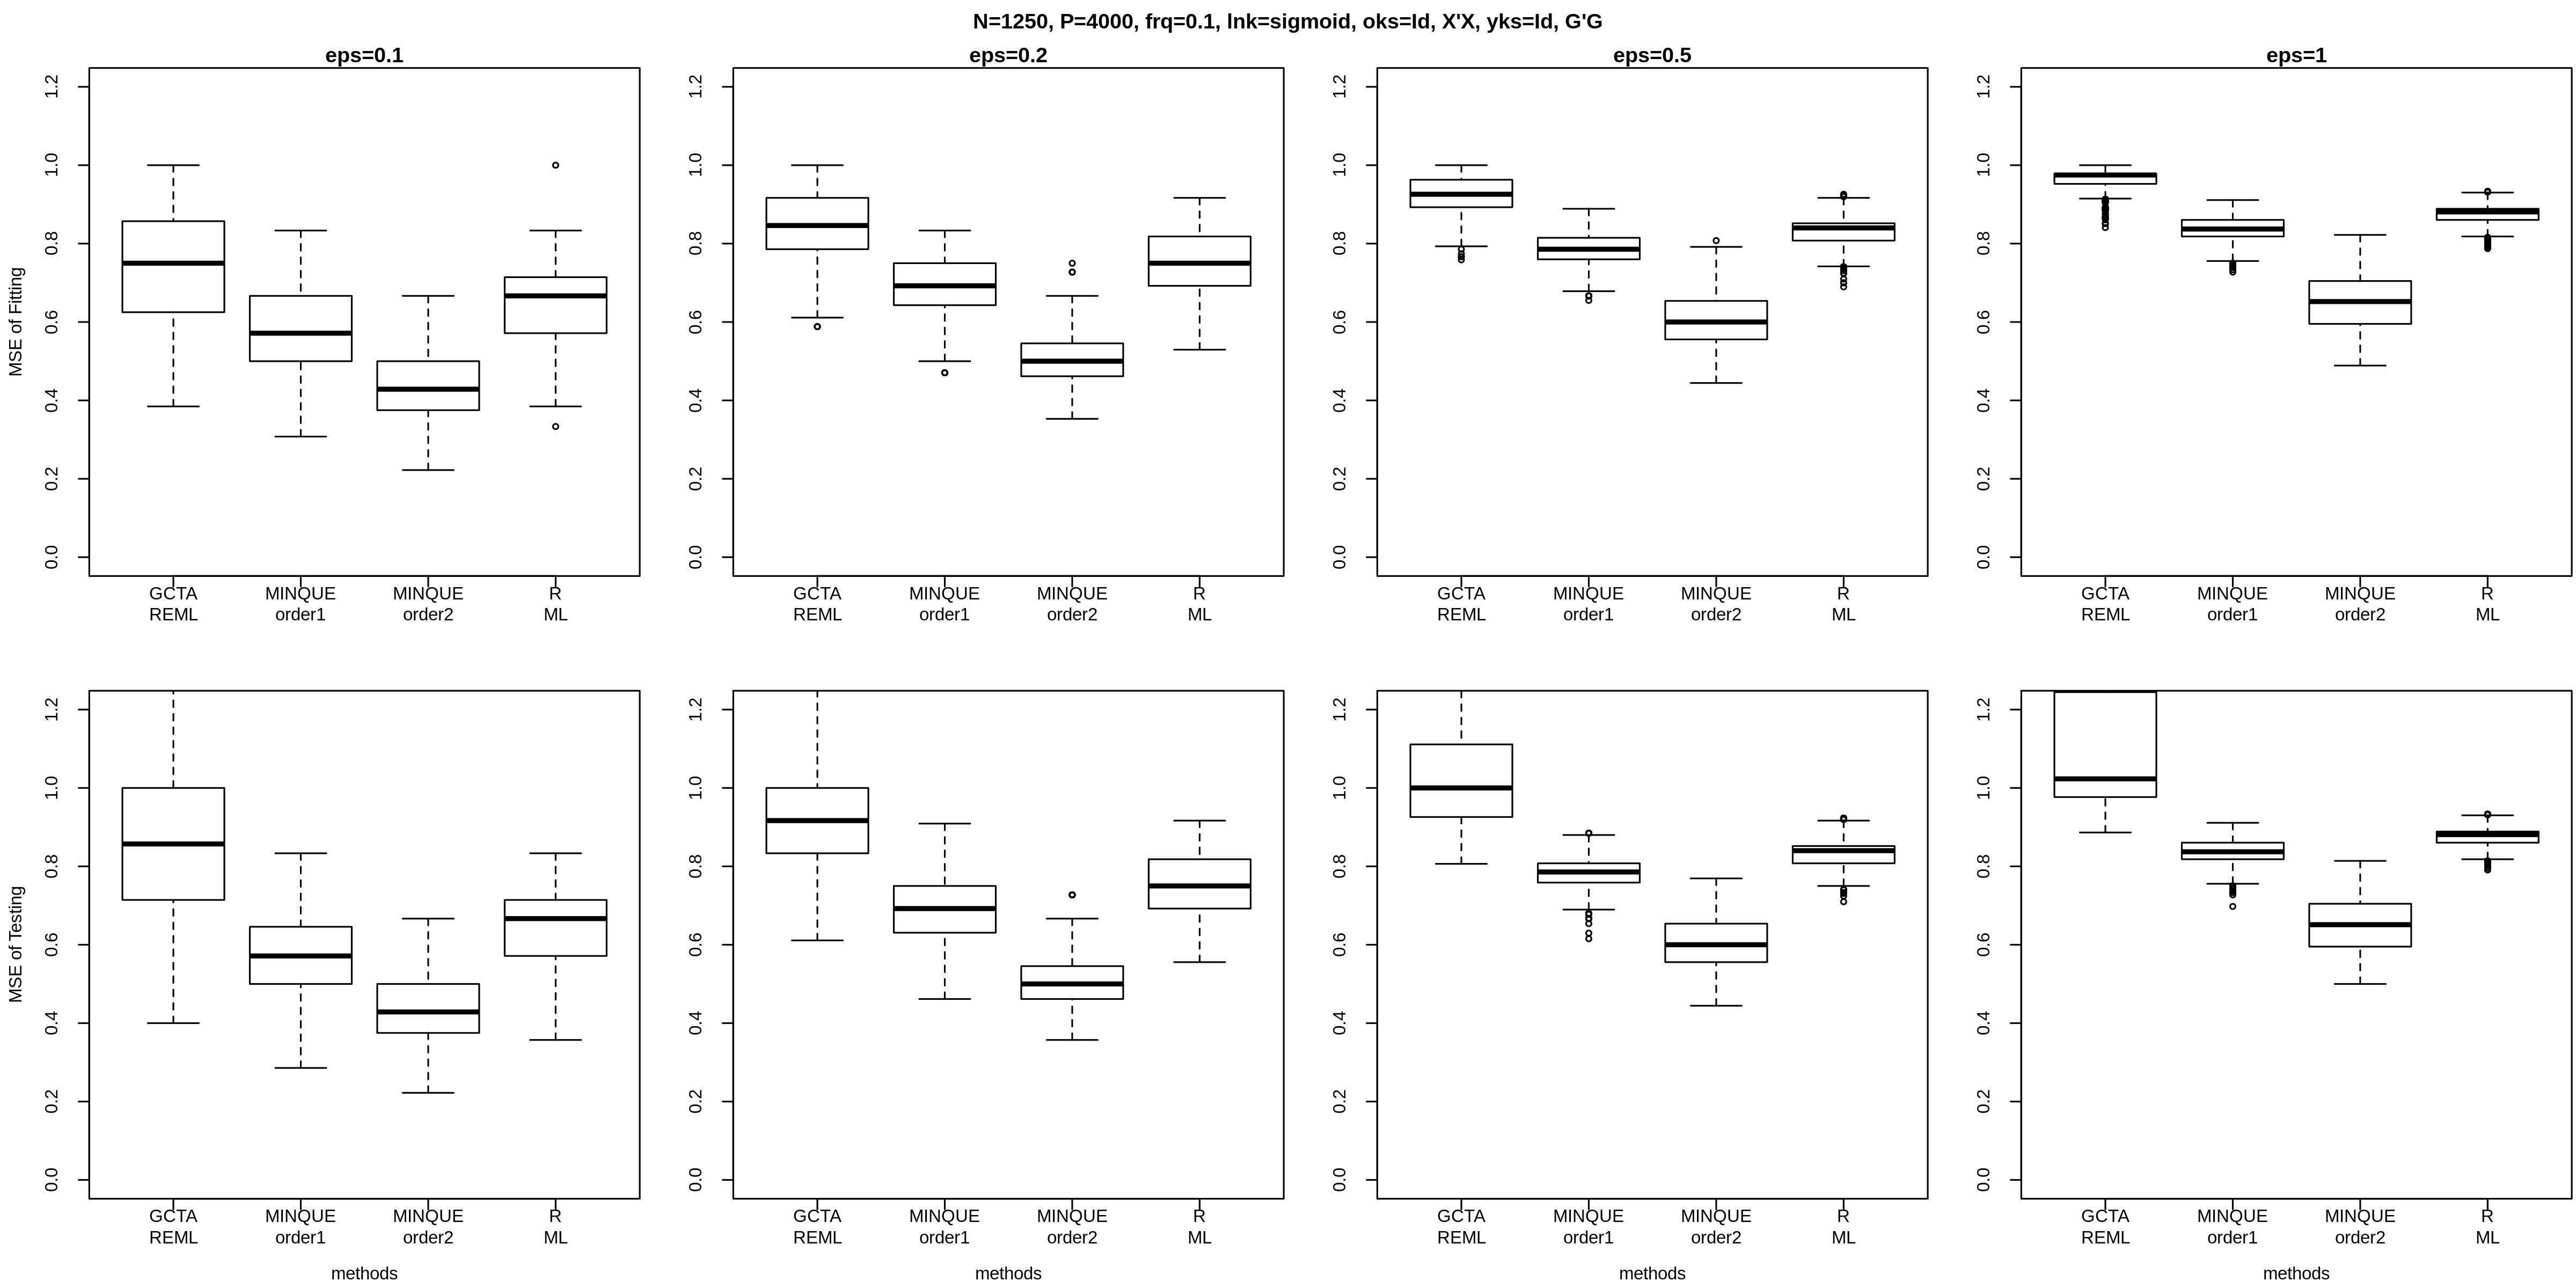
\includegraphics[width=1.00\linewidth]{s02_bxp.png}\end{figure}
\end{frame}
\begin{frame}{EXP 02: sigmoid distortion of $\vy$, RTM}
  \begin{figure}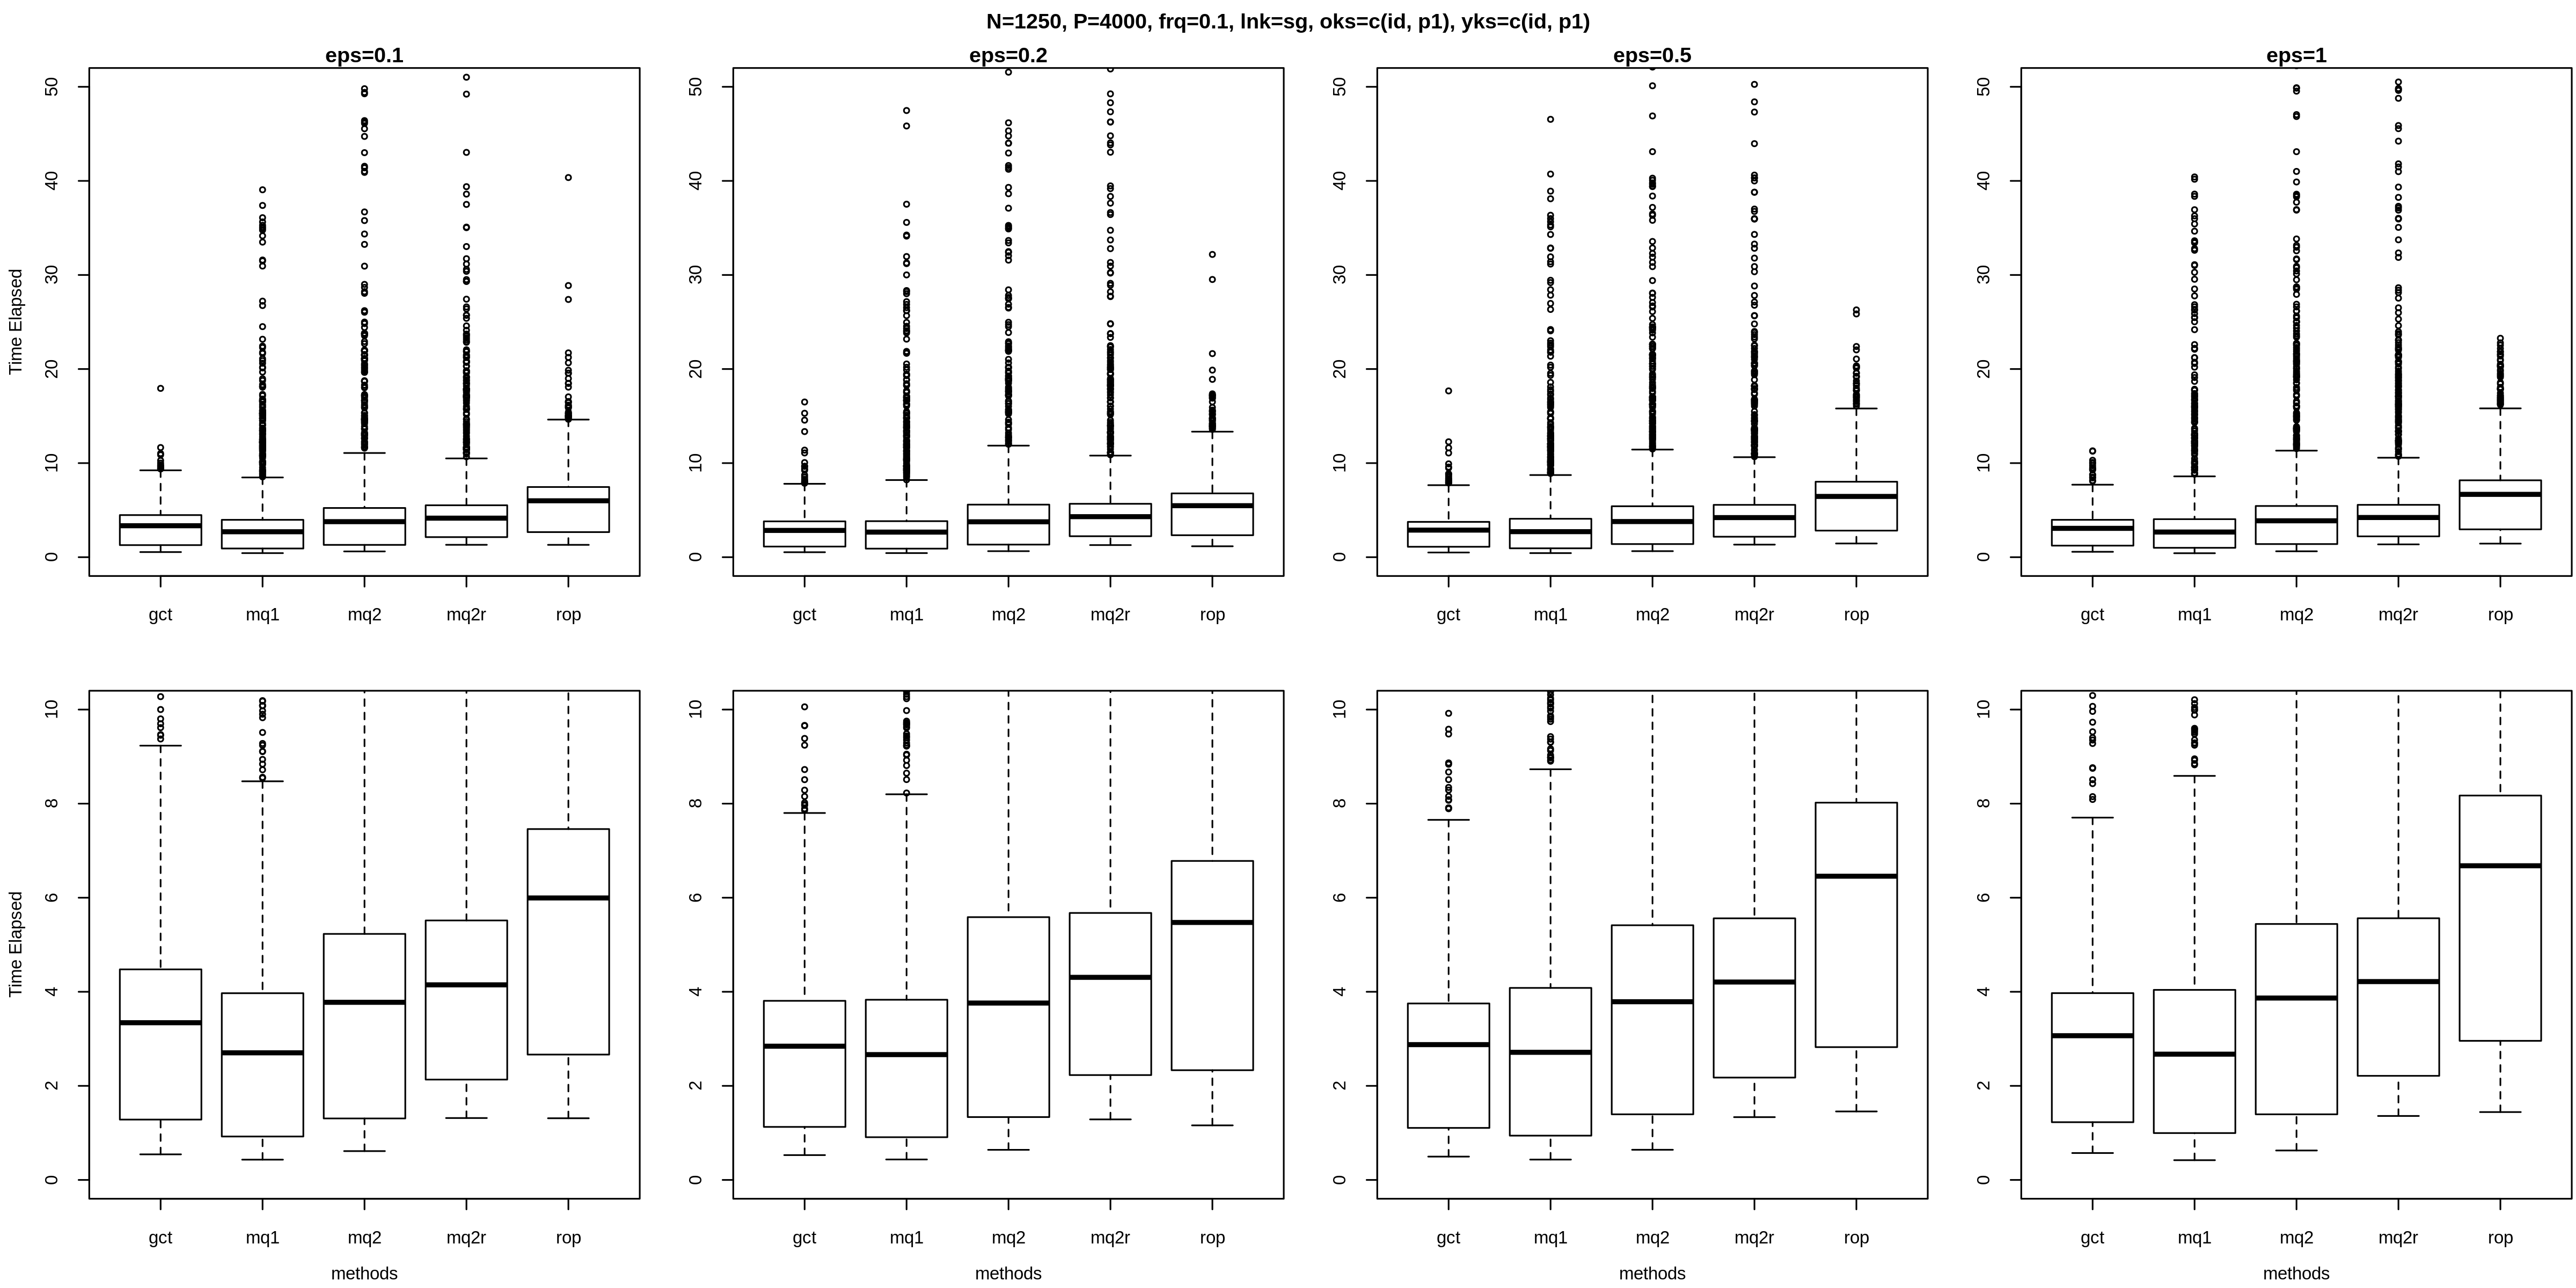
\includegraphics[width=1.00\linewidth]{t02_bxp.png}\end{figure}
\end{frame}
%---------------------------------------------------------
\begin{frame}{EXP 03: sin distortion of $1\pi\vy$, MSE}
  \begin{figure}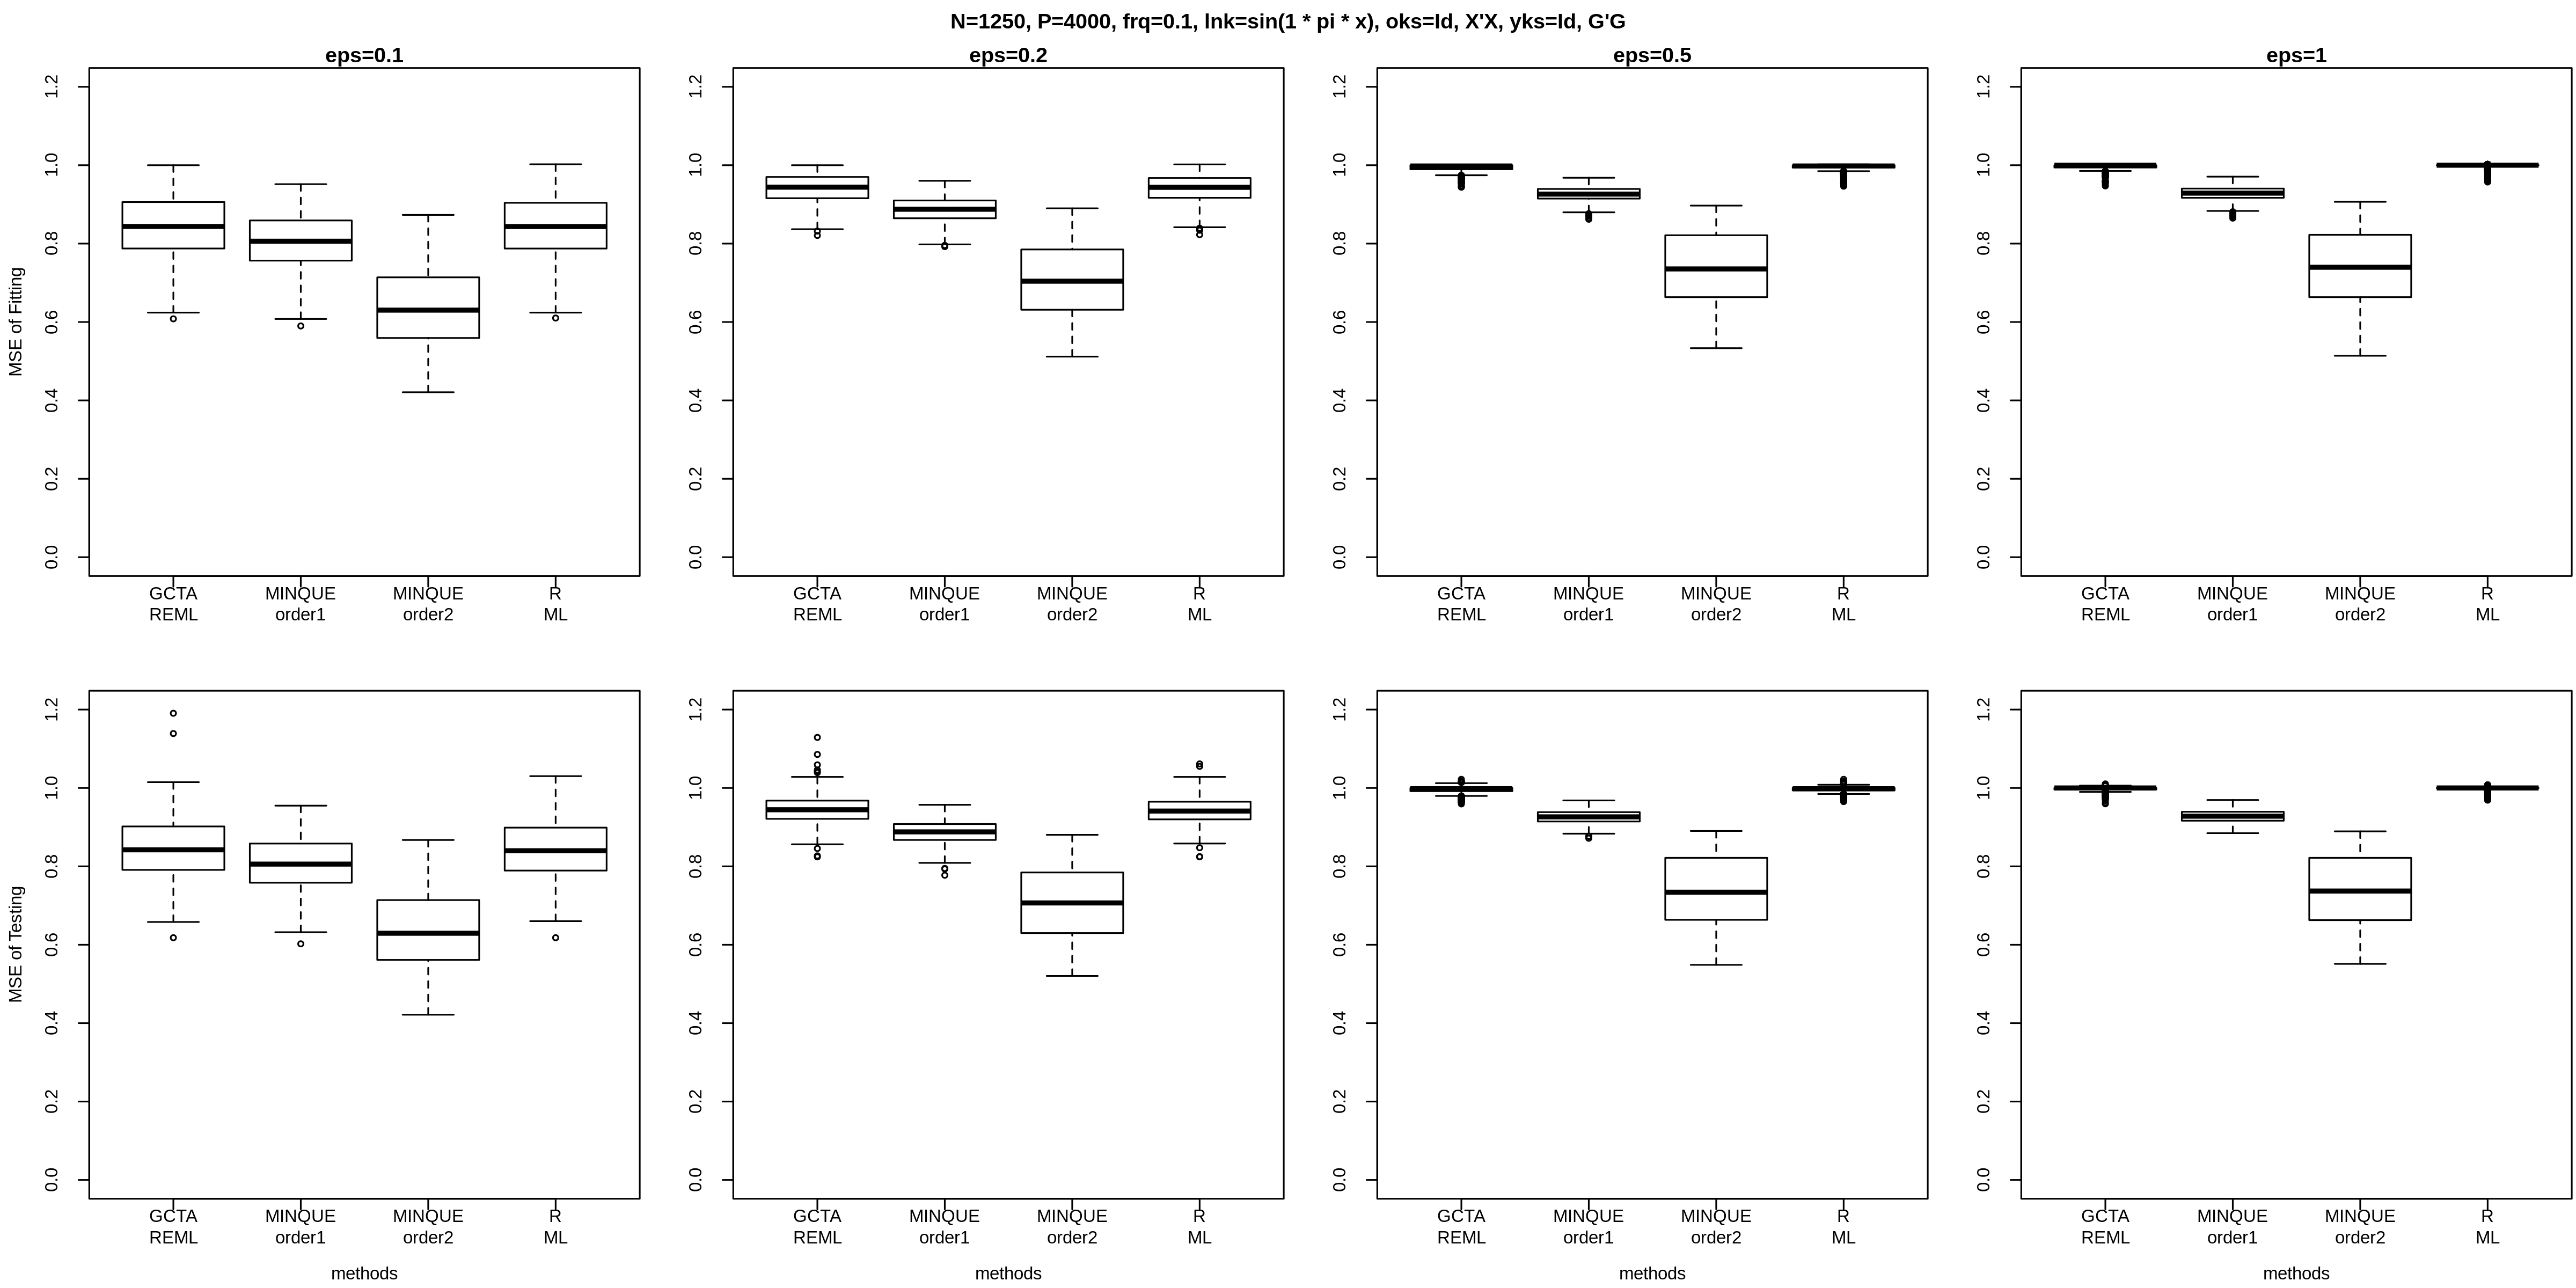
\includegraphics[width=1.00\linewidth]{s03_bxp.png}\end{figure}
\end{frame}
\begin{frame}{EXP 03: sin distortion of $1\pi\vy$, RTM}
  \begin{figure}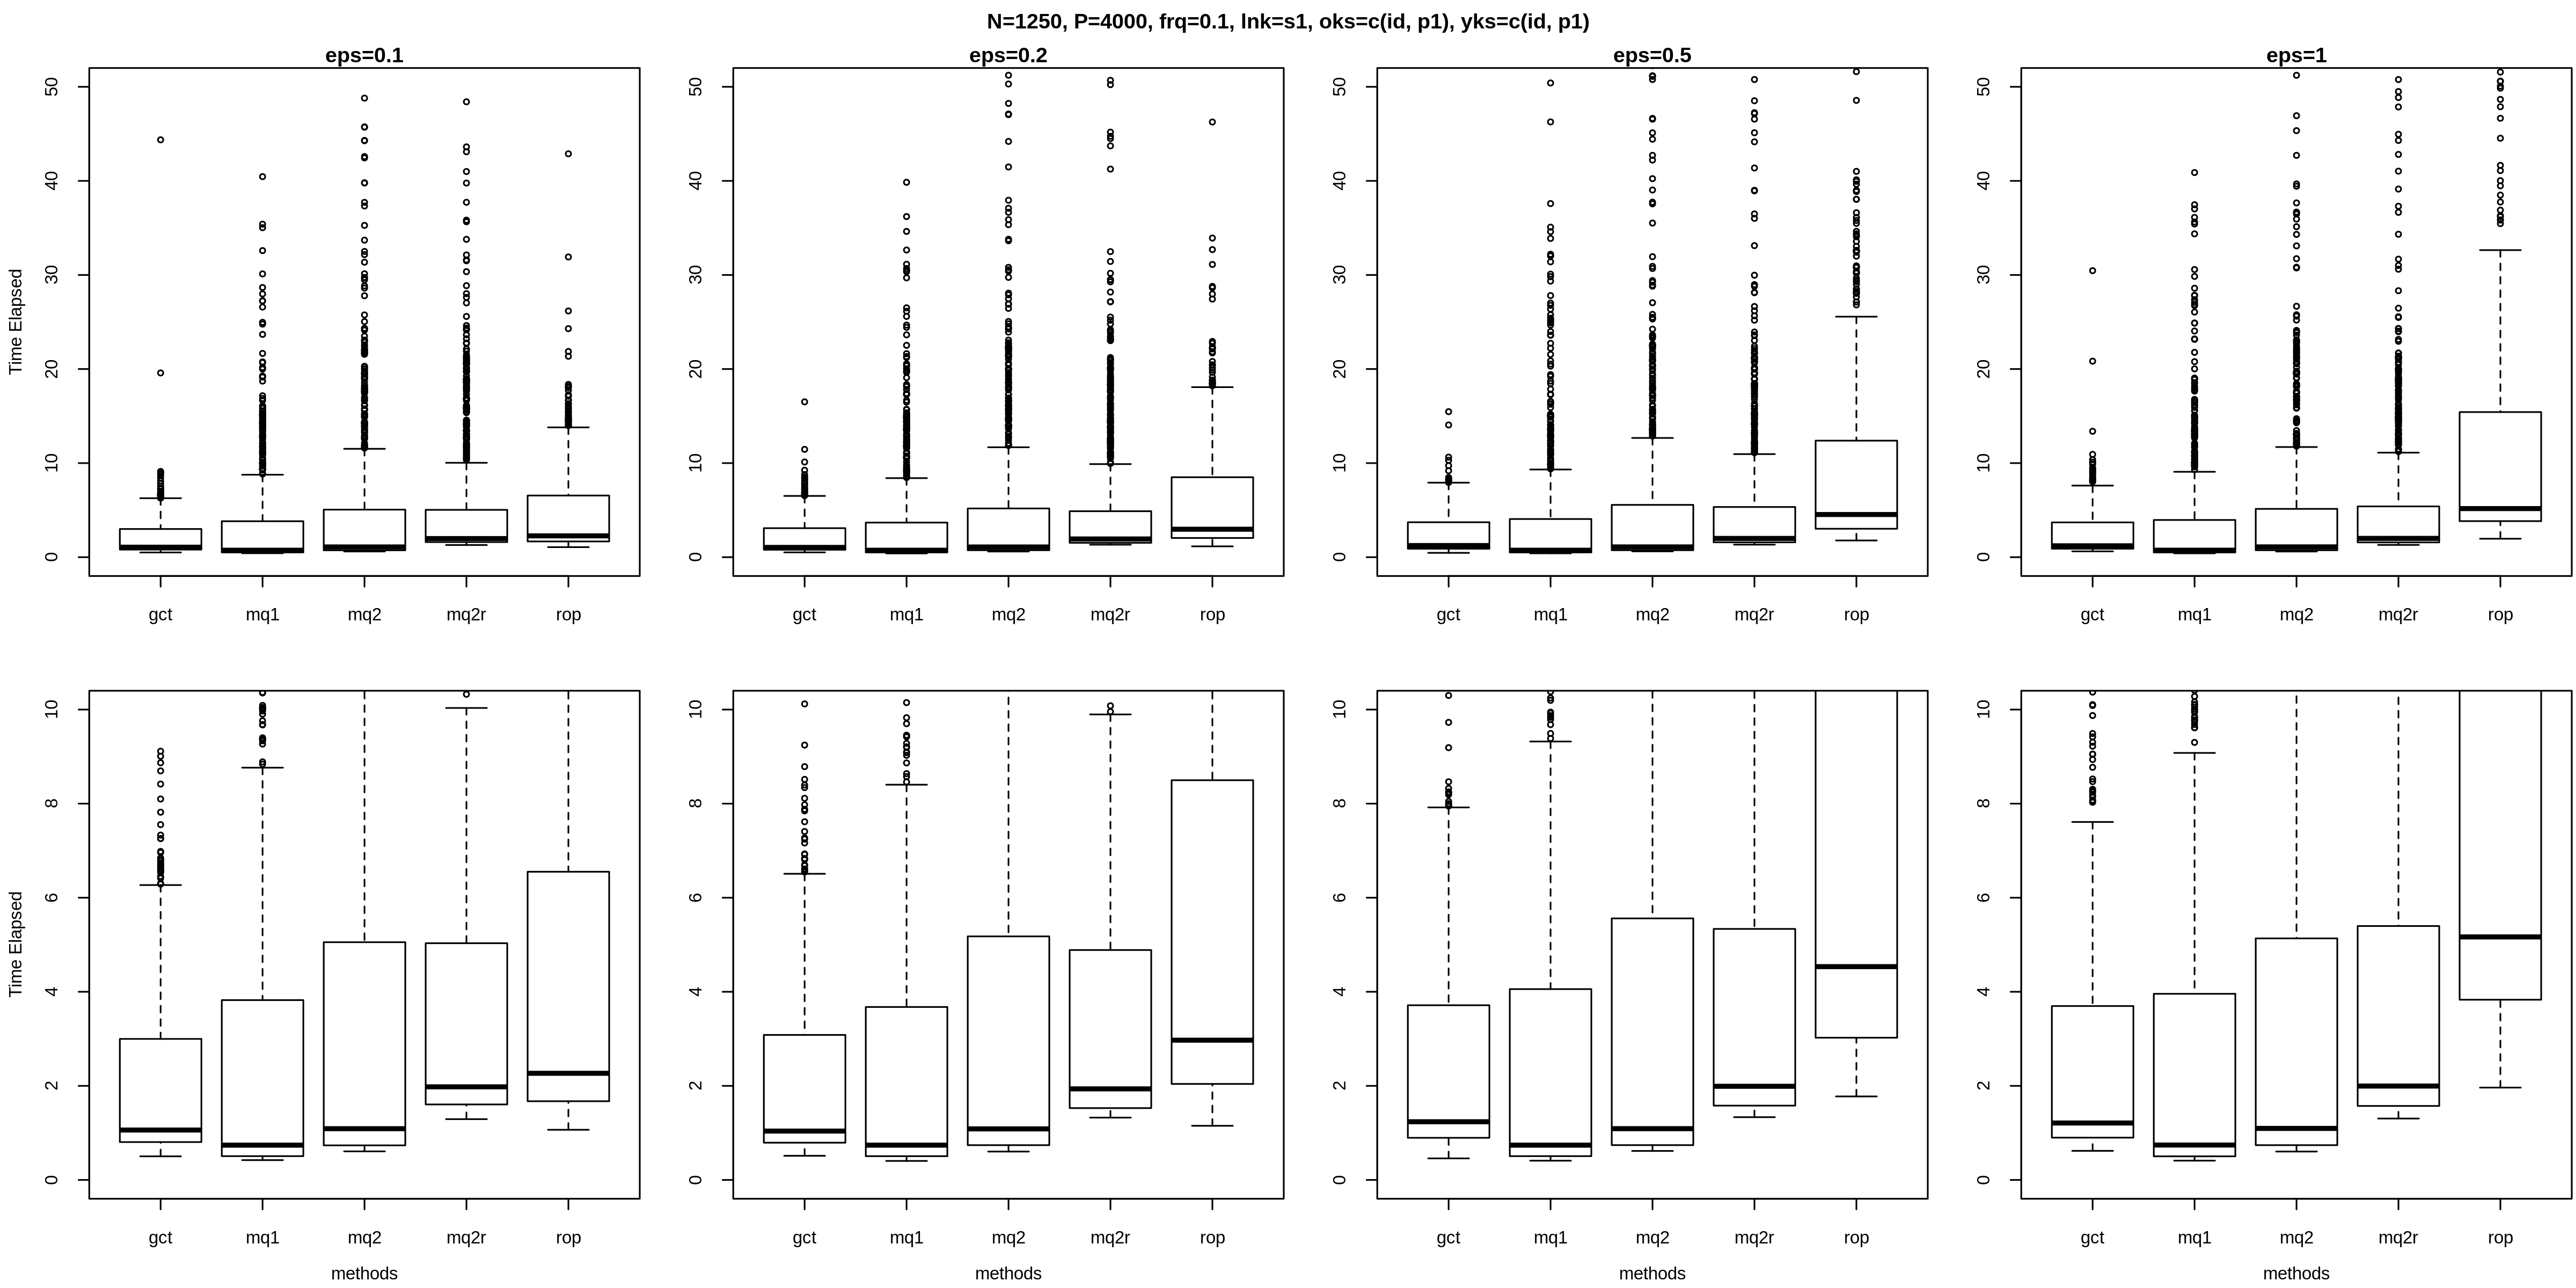
\includegraphics[width=1.00\linewidth]{t03_bxp.png}\end{figure}
\end{frame}
%---------------------------------------------------------
\begin{frame}{EXP 04: sin distortion of $2\pi\vy$, MSE}
  \begin{figure}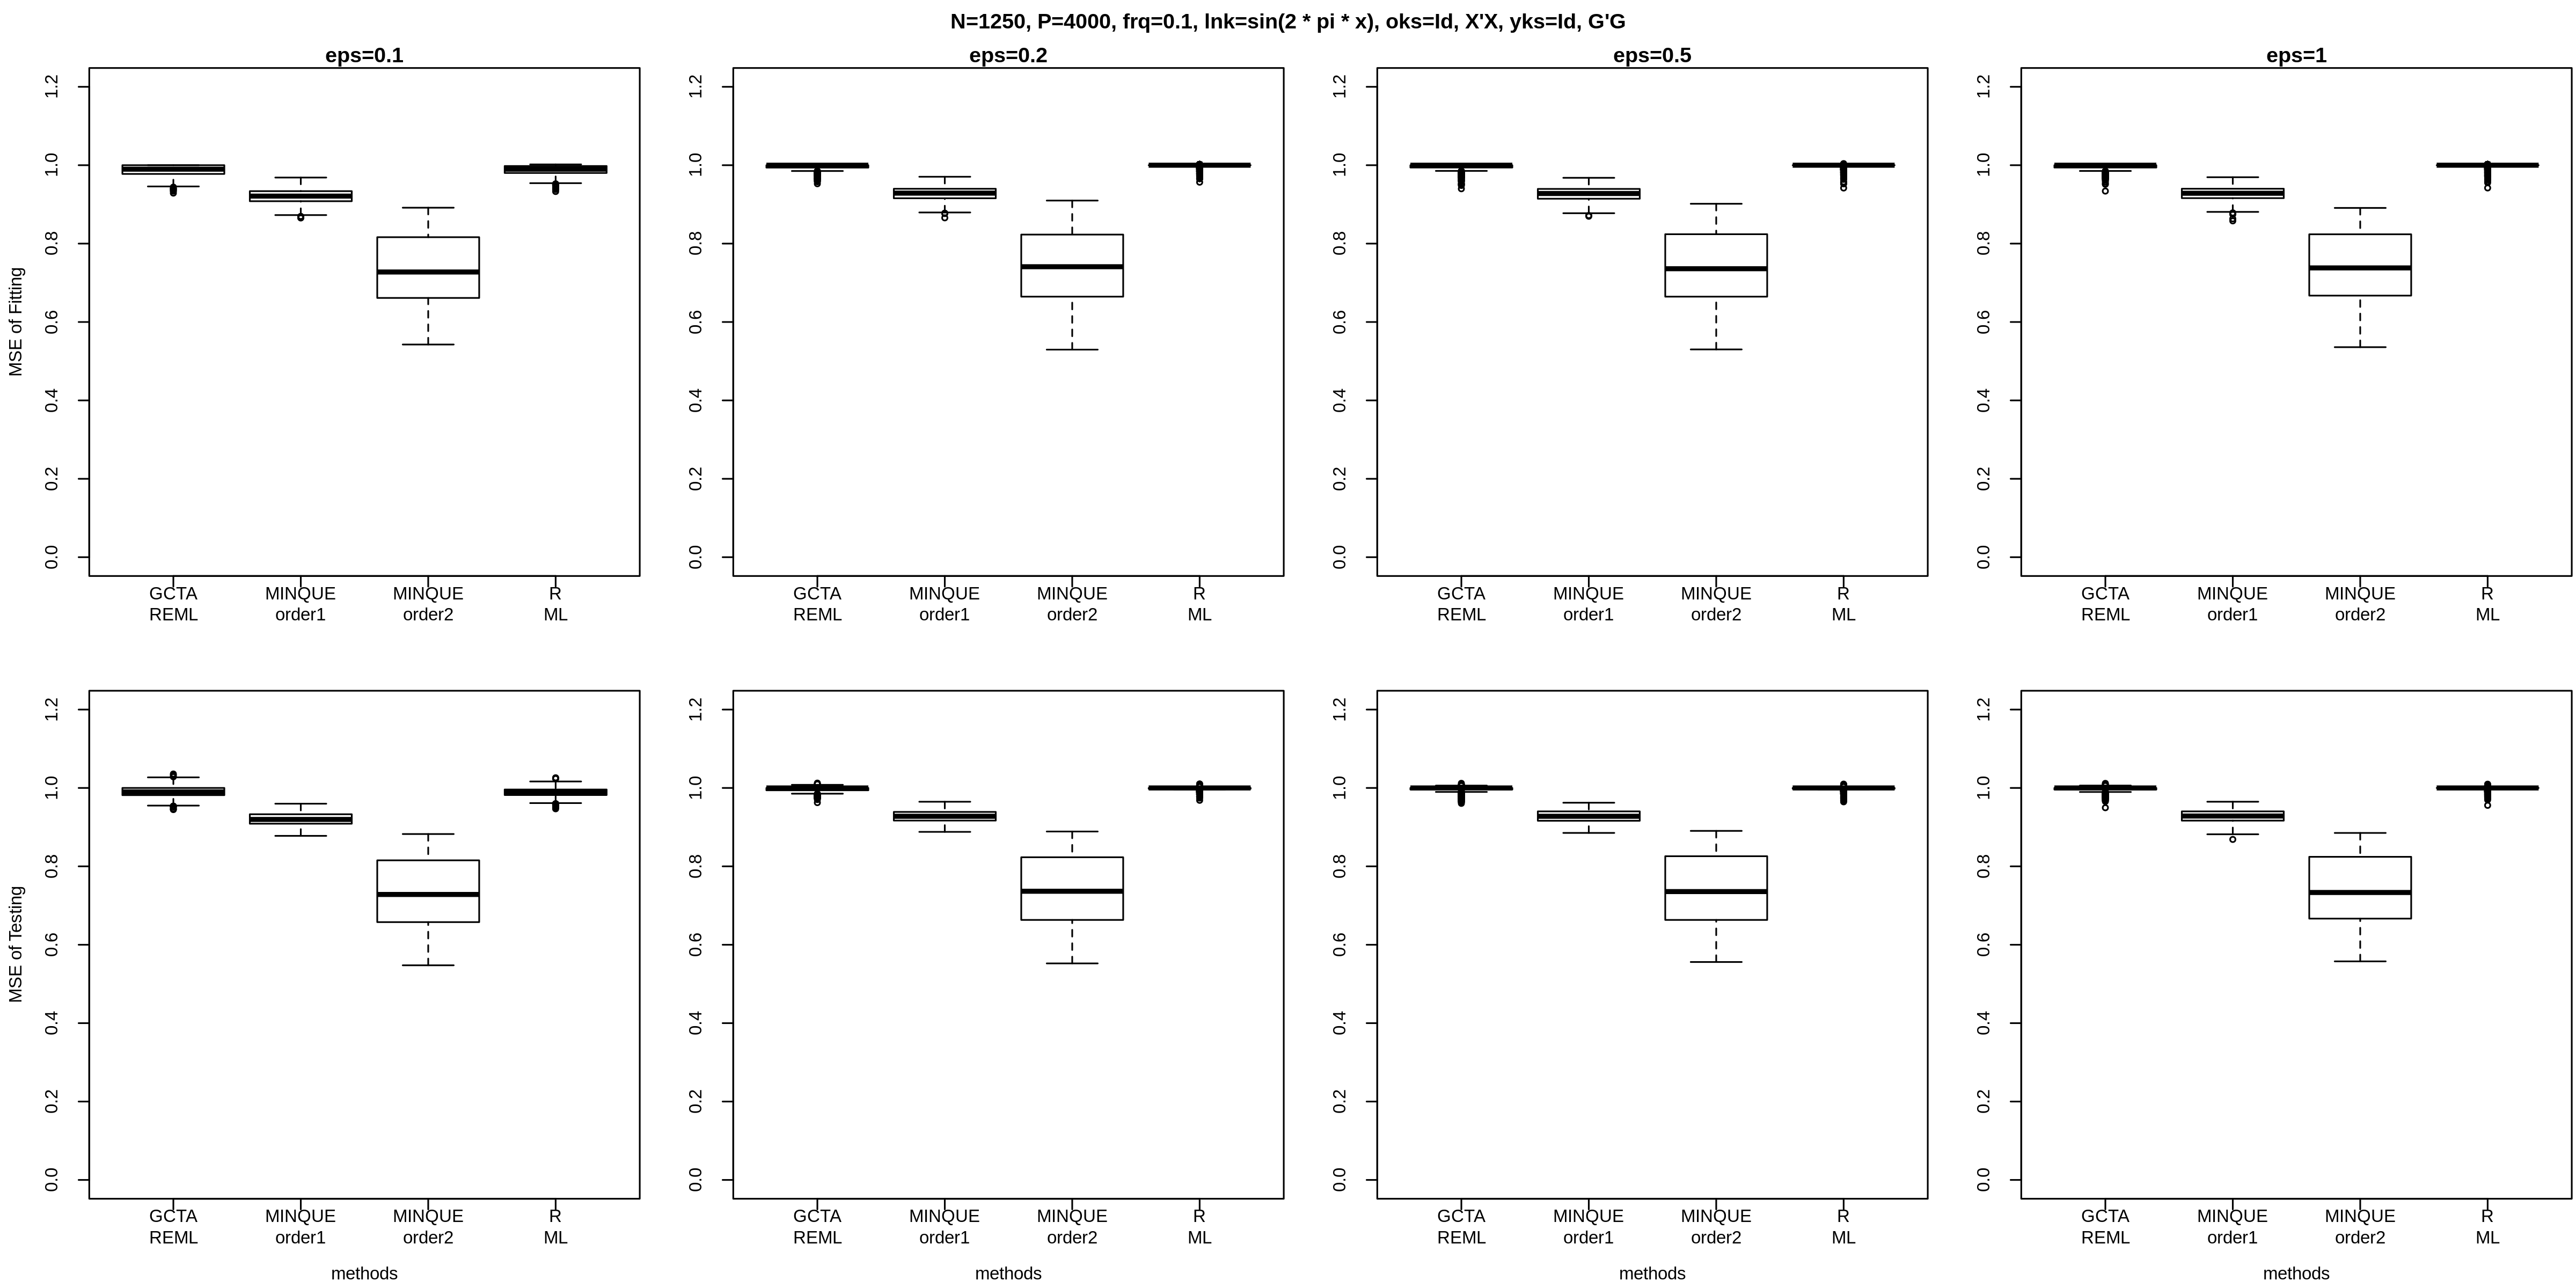
\includegraphics[width=1.00\linewidth]{s04_bxp.png}\end{figure}
\end{frame}
\begin{frame}{EXP 04: sin distortion of $2\pi\vy$, RTM}
  \begin{figure}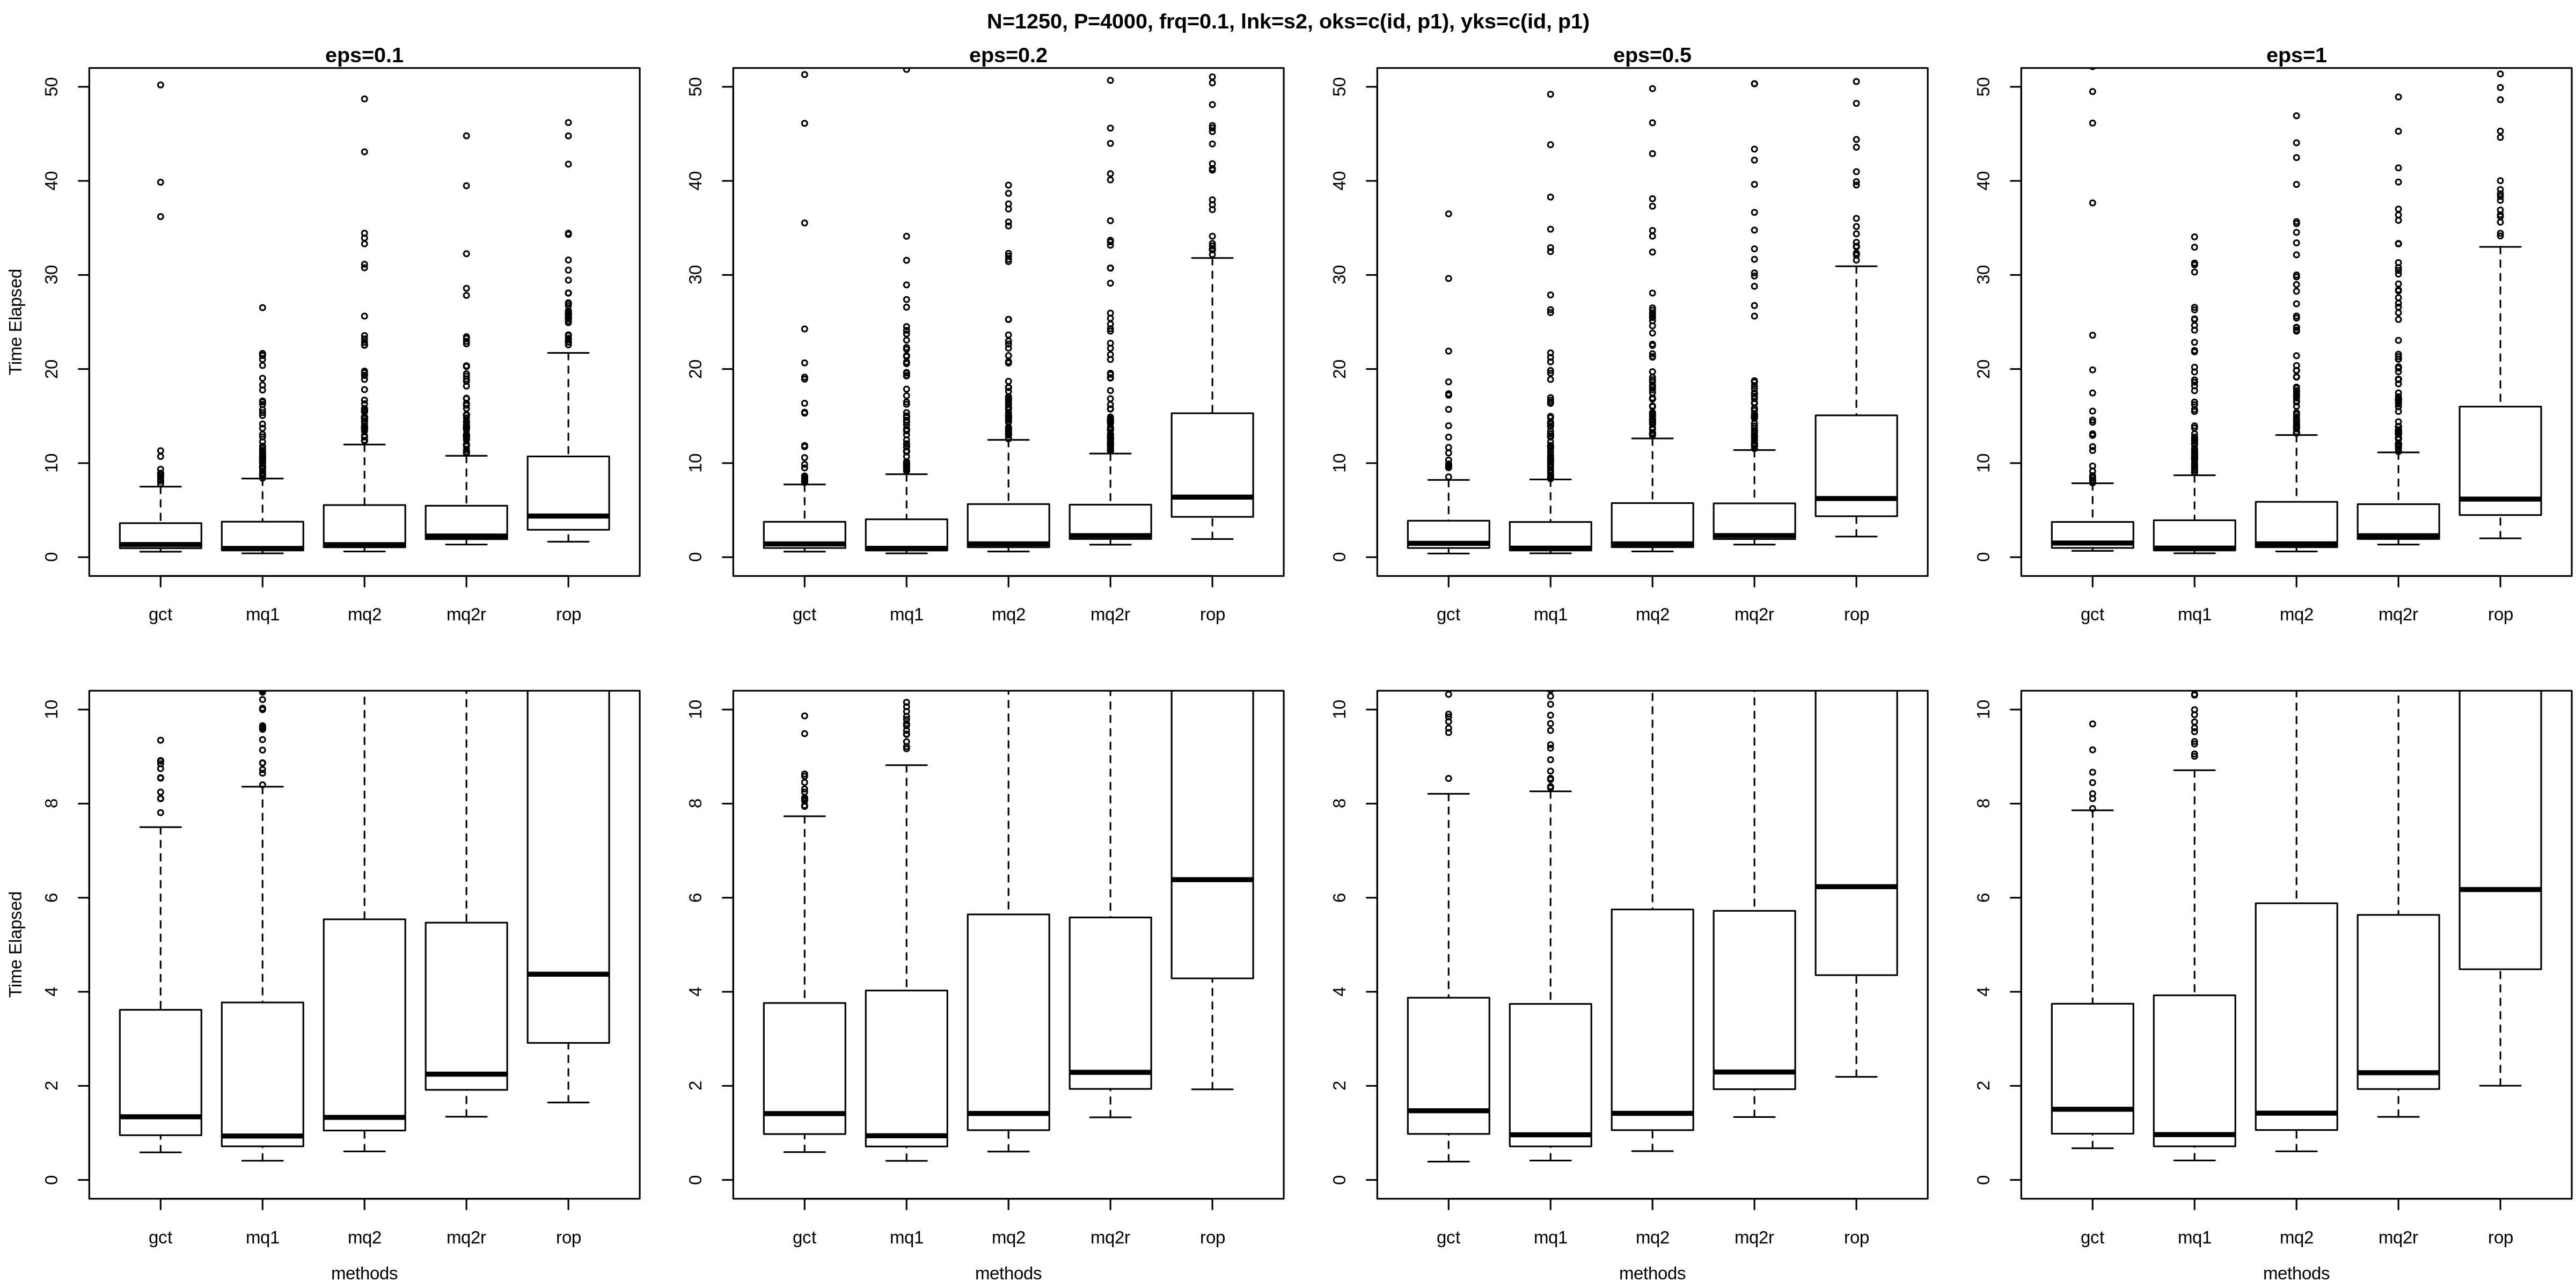
\includegraphics[width=1.00\linewidth]{t04_bxp.png}\end{figure}
\end{frame}
%---------------------------------------------------------
\section{Speculation}
\frametitle{Speculation:}
\begin{frame}
  \begin{itemize}
  \item MINQUE, especially polynomial MINQUE, is robust against
    mis-specified covariance structure and non-normal dependent
    variable due to distortion.
  \item the wide spread of running time may be due to the variability
    in the difficulty of inverting $\xv$ matrix under different 
    circumstances.
  \item in terms of medium running time, the current Rcpp implementation
    of MINQUE is comparable to GCTA and out-perform the rest.x
  \end{itemize}
\end{frame}
% ---------------------------------------------------------
\end{document}
